\section{(Parallel) Louvain Algorithm}

\begin{frame}{Louvain Algorithm (serial)}{}
\begin{enumerate}
 \item<1-> Every vertex starts in own cluster. Also assign arbitrary order.
 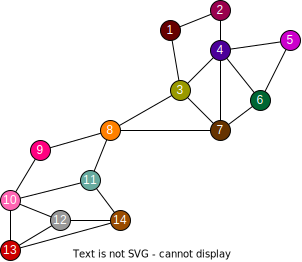
\includegraphics[scale=0.45]{220523_distparallel_louvainstart.drawio.svg}
 \item<2-> Traverse vertices sequentially. For every vertex:
 \begin{enumerate}
   \item<3-> Does clustering get better if the vertex gets assigned to \textbf{neighbor clusters}? ($\Delta Q$)
   \item<4-> \textbf{Assign} vertex to neighbor vertex' cluster that improves clustering the most.
 \end{enumerate}
 \item<5-> Collapse clusters into \emph{Super Nodes}. Repeat till convergence.
\end{enumerate}
\end{frame}

\begin{frame}{How to make this parallel?}
  \begin{itemize}
    \item<1-> Basic idea: traverse vertices \textbf{in parallel} without locks.
    \item<2-> Use a set of heuristics to \textbf{avoid these challenges}:
    \begin{enumerate}
      \item<3-> Nodes moving into their respective clusters \textbf{concurrently}.
      \item<4-> Clustering getting worse due to lacking information.
    \end{enumerate}
  \end{itemize}
\end{frame}

\begin{frame}[label=louvain-par-challenge]{Louvain Algorithm (parallelization challenges)}
  \begin{enumerate}
  \item<1-> Consider thread $b$ is currently on $C_b$ and thread $c$ is on $C_b$:
  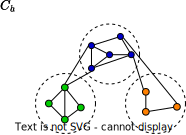
\includegraphics[scale=0.7]{220523_distparallel.drawio.fig1a.svg}

  \item<2-> What actually happens:
  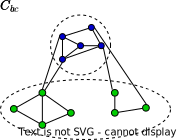
\includegraphics[scale=0.7]{220523_distparallel.drawio.fig1b.svg}
  \end{enumerate}
\end{frame}

\begin{frame}{Louvain Algorithm (parallel heuristic: coloring)}
  \begin{itemize}
    \item<1-> Consider a distance-1 coloring of a graph:
    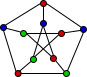
\includegraphics[scale=1.5]{220523_distparallel.drawio.coloring.svg}
    \item<2-> \textbf{Idea:} only process one color at a time in parallel.
    \item<3-> Avoids vertex swaps, but what about negative modularity gain?
  \end{itemize}
\end{frame}

\begin{frame}{Louvain Algorithm (parallel heuristic: minimum label)}
  \begin{itemize}
    \item<1-> How to prevent vertex swapping and negative modularity gain \textbf{initially}?
    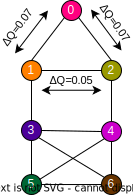
\includegraphics[scale=0.8]{220523_distparallel.drawio.singlet_minimum_label.svg}
    \item<2-> \textbf{Idea:} only execute move if $l(v) < l(w)$.
  \end{itemize}
\end{frame}